\begin{figure}
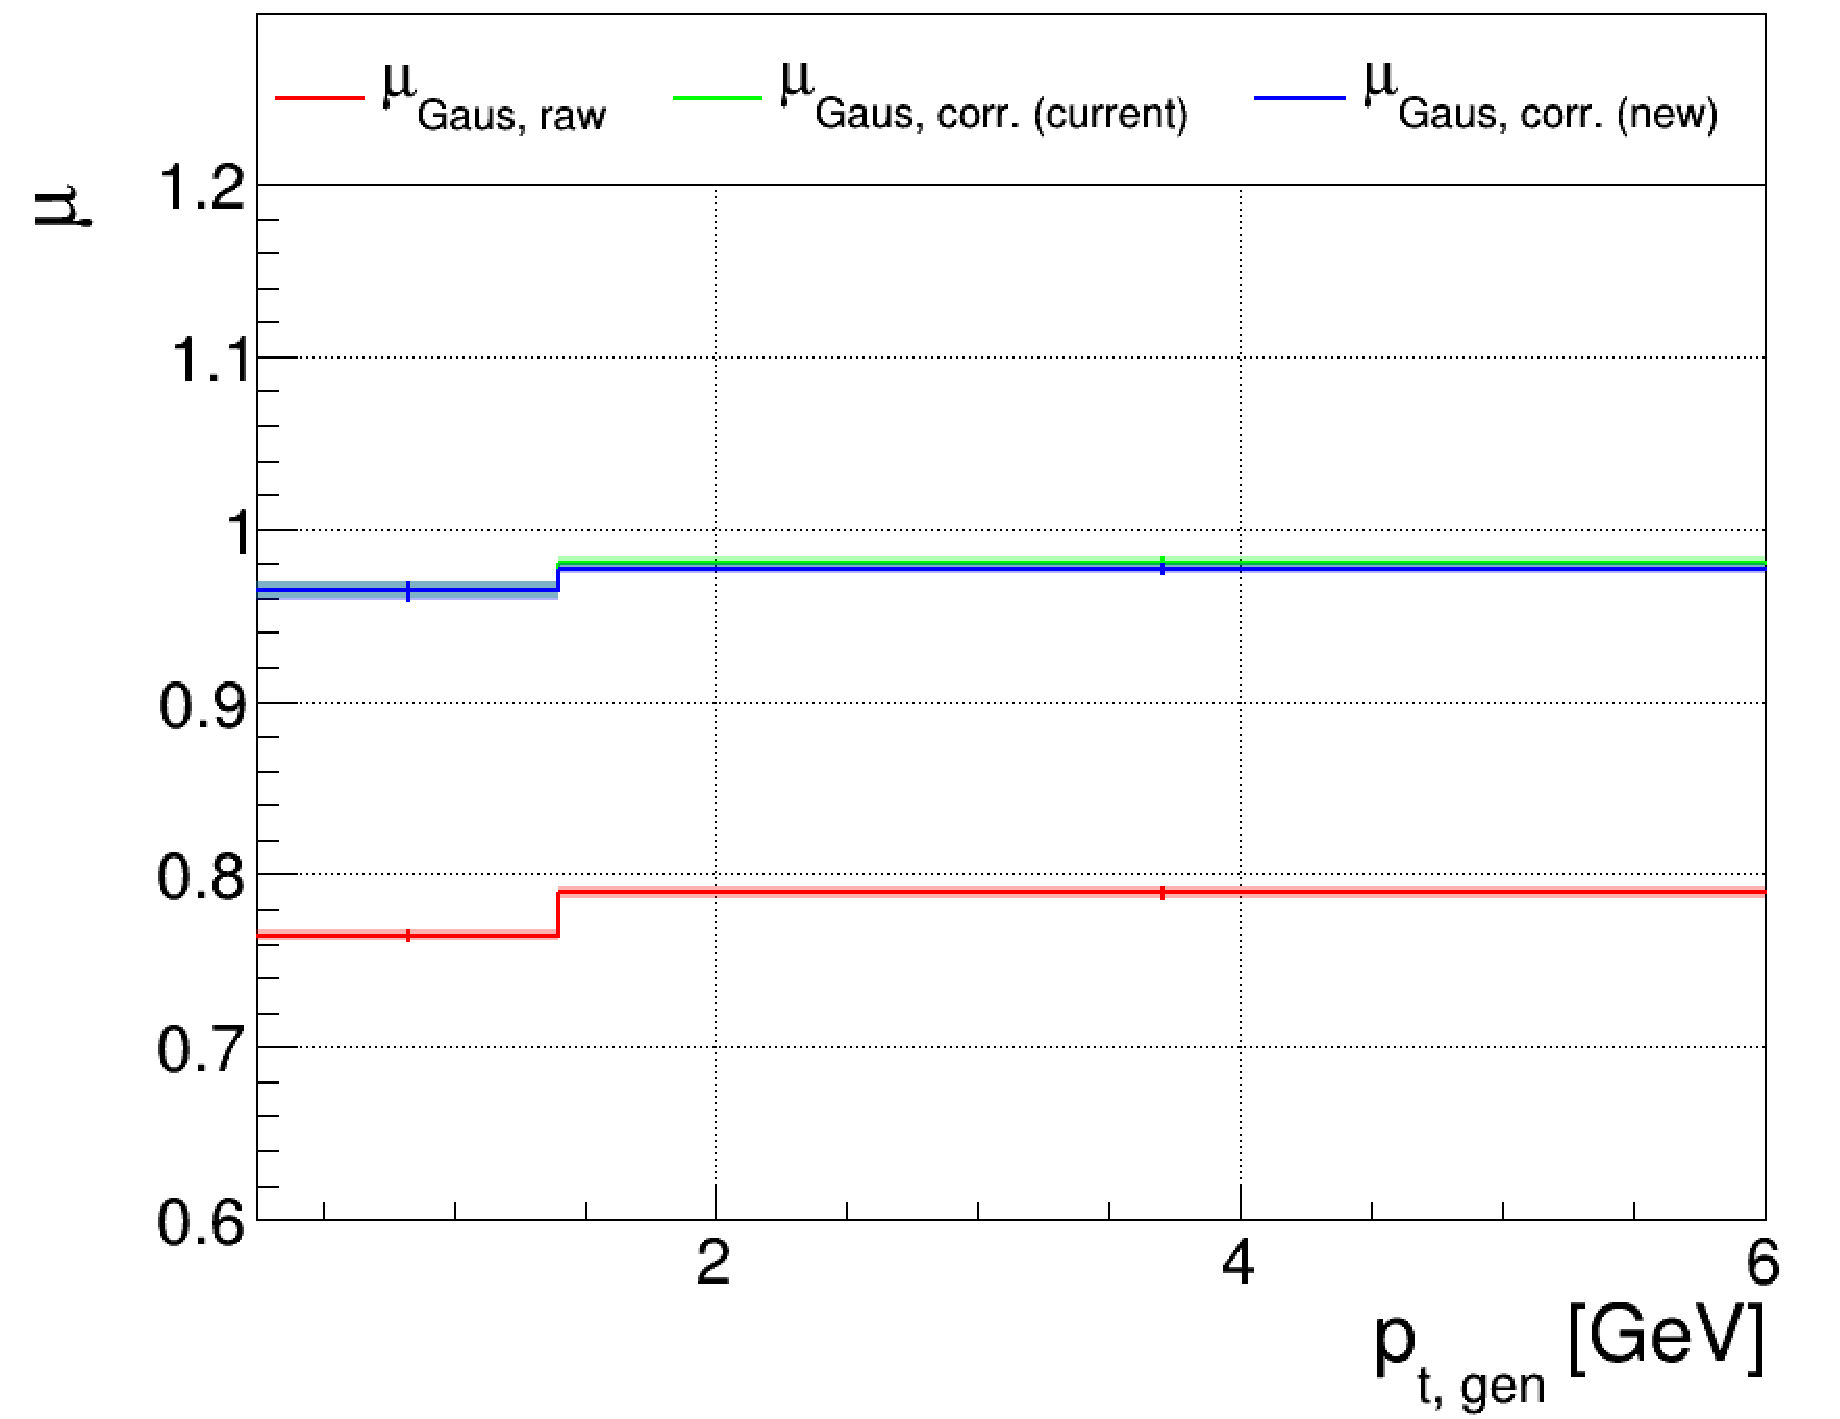
\includegraphics[width=0.495\textwidth]{./plots_pdf/ECAL_plots/plotsPU/EE/ZS/pdf/GENPT/EEZS_GENPT_0000_0006_MuOverBins.pdf}
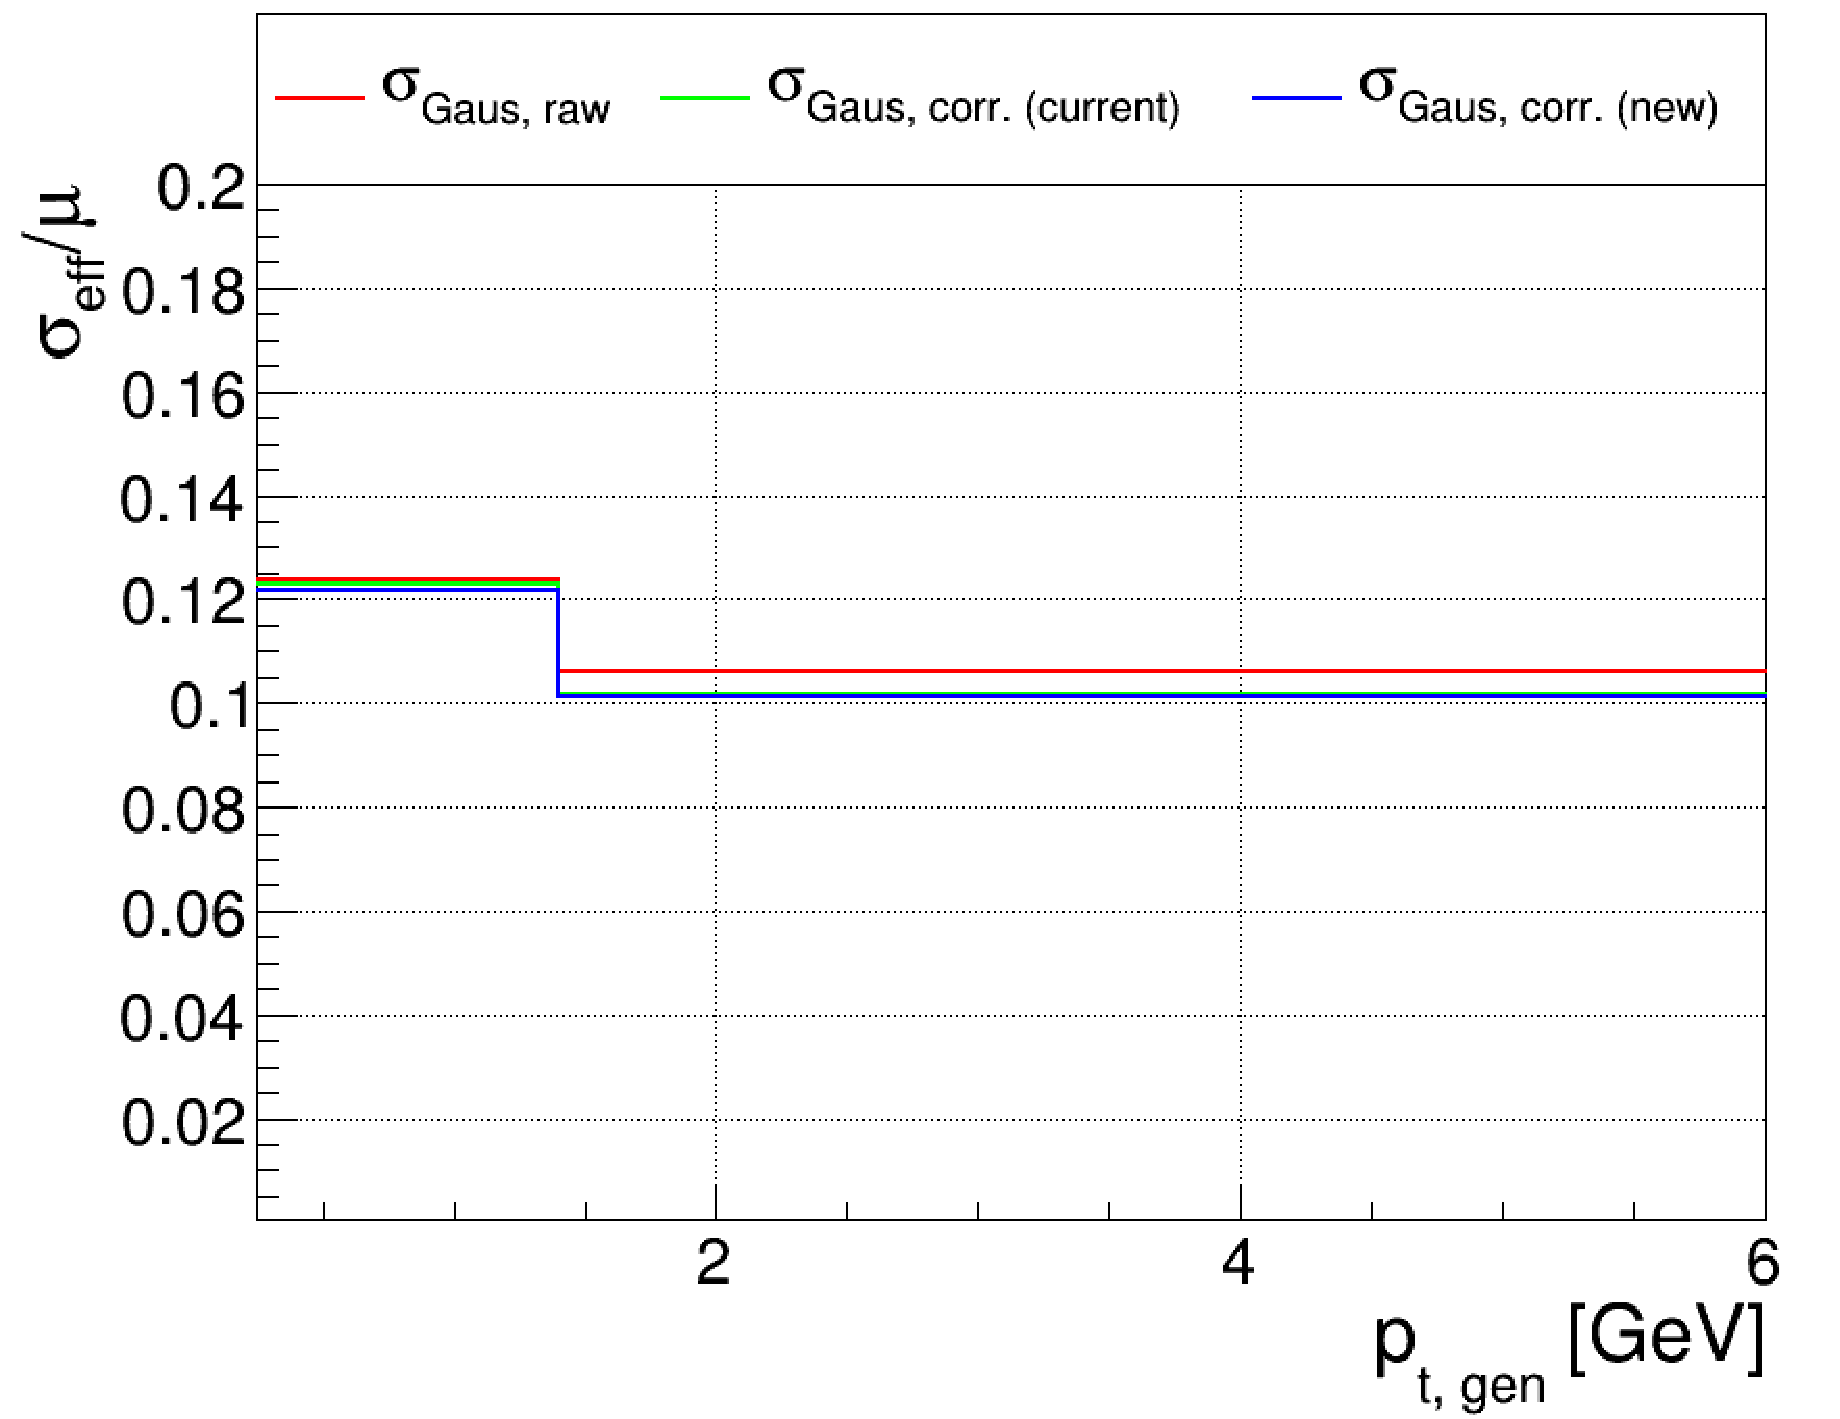
\includegraphics[width=0.495\textwidth]{./plots_pdf/ECAL_plots/plotsPU/EE/ZS/pdf/GENPT/EEZS_GENPT_0000_0006_EffSigmaOverBins.pdf}

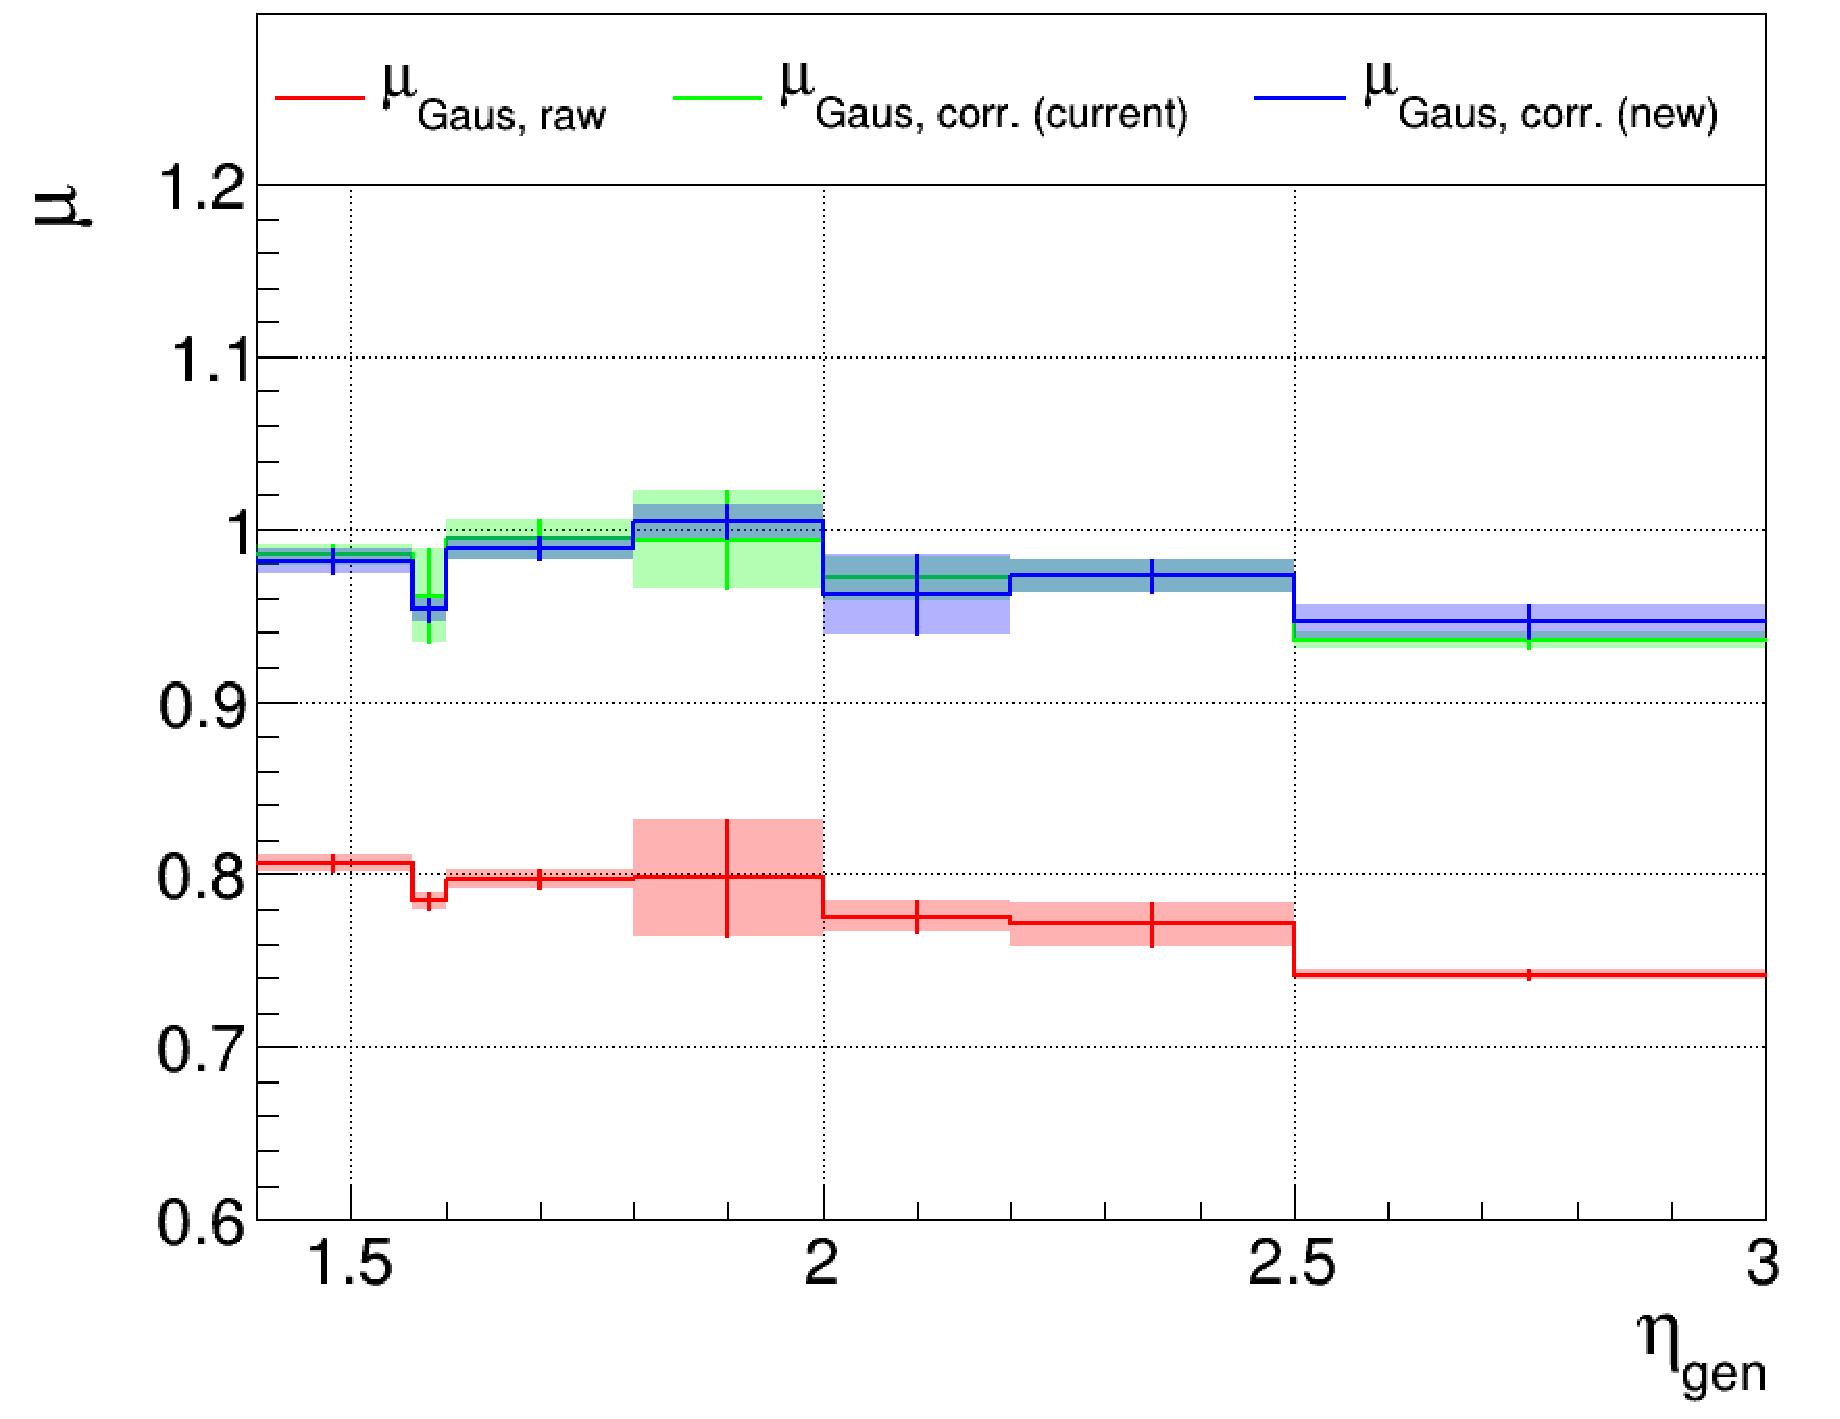
\includegraphics[width=0.495\textwidth]{./plots_pdf/ECAL_plots/plotsPU/EE/ZS/pdf/GENETA/EEZS_GENETA_0000_0006_MuOverBins.pdf}
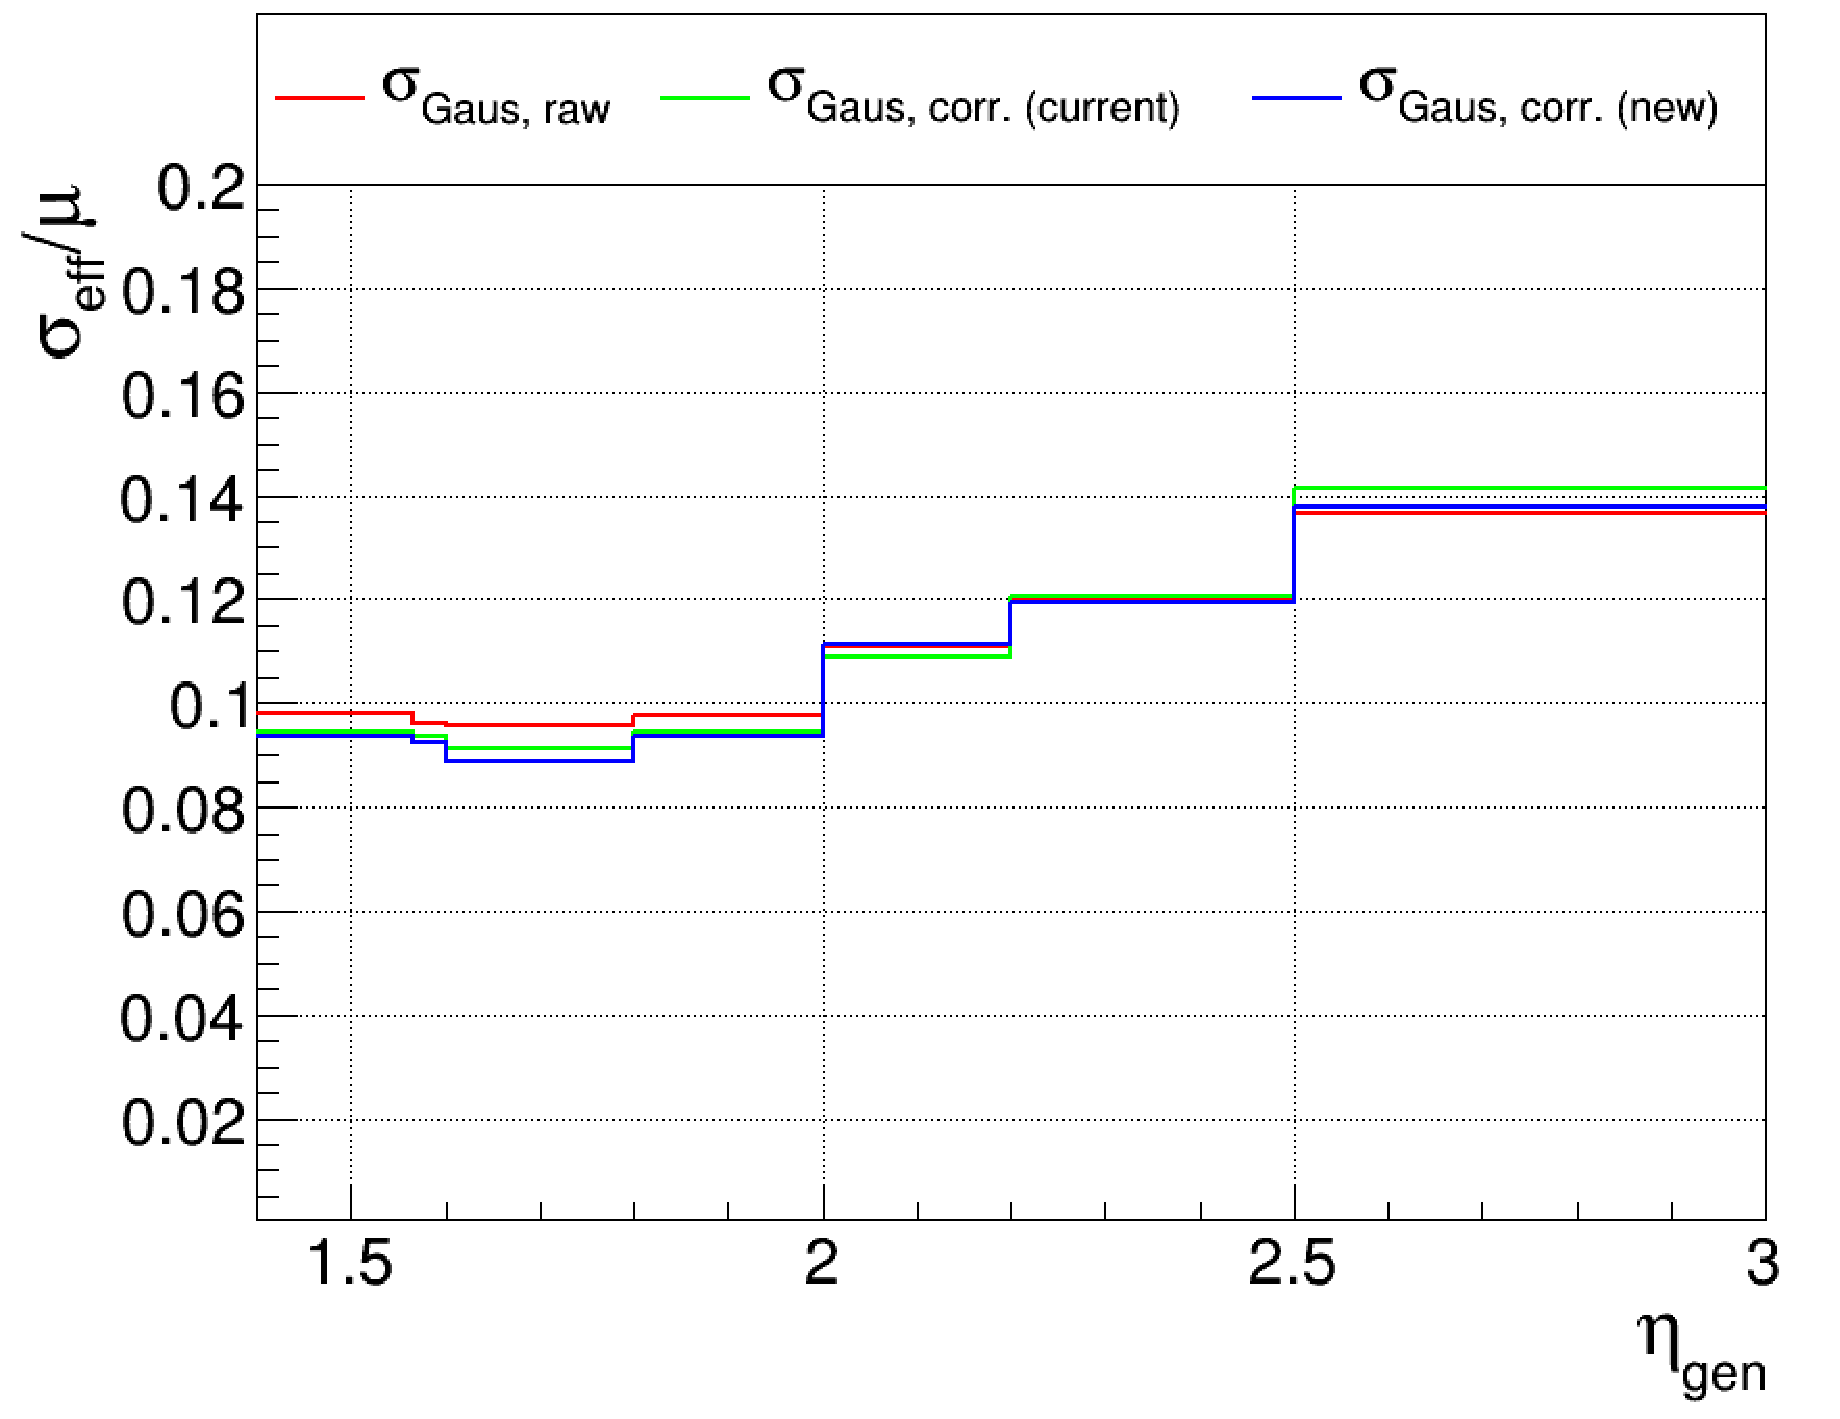
\includegraphics[width=0.495\textwidth]{./plots_pdf/ECAL_plots/plotsPU/EE/ZS/pdf/GENETA/EEZS_GENETA_0000_0006_EffSigmaOverBins.pdf}

\caption[$\mu$ ($\sigma_\mathrm{eff}$) vs. \pt of PF ECAL cluster - EE ZS readout PU scenario]{Mean response (resolution) defined by raw PF ECAL clusters (red), the calibration derived earlier in Run~3 based on 126X (green), and the new correction from the 2024 simulation sample based on 133X (blue).\pt 0--6\GeV in EE region ZS readout PU scenario.}
\label{fig:PU_EEZS}
\end{figure}

%% %\begin{figure}
%% 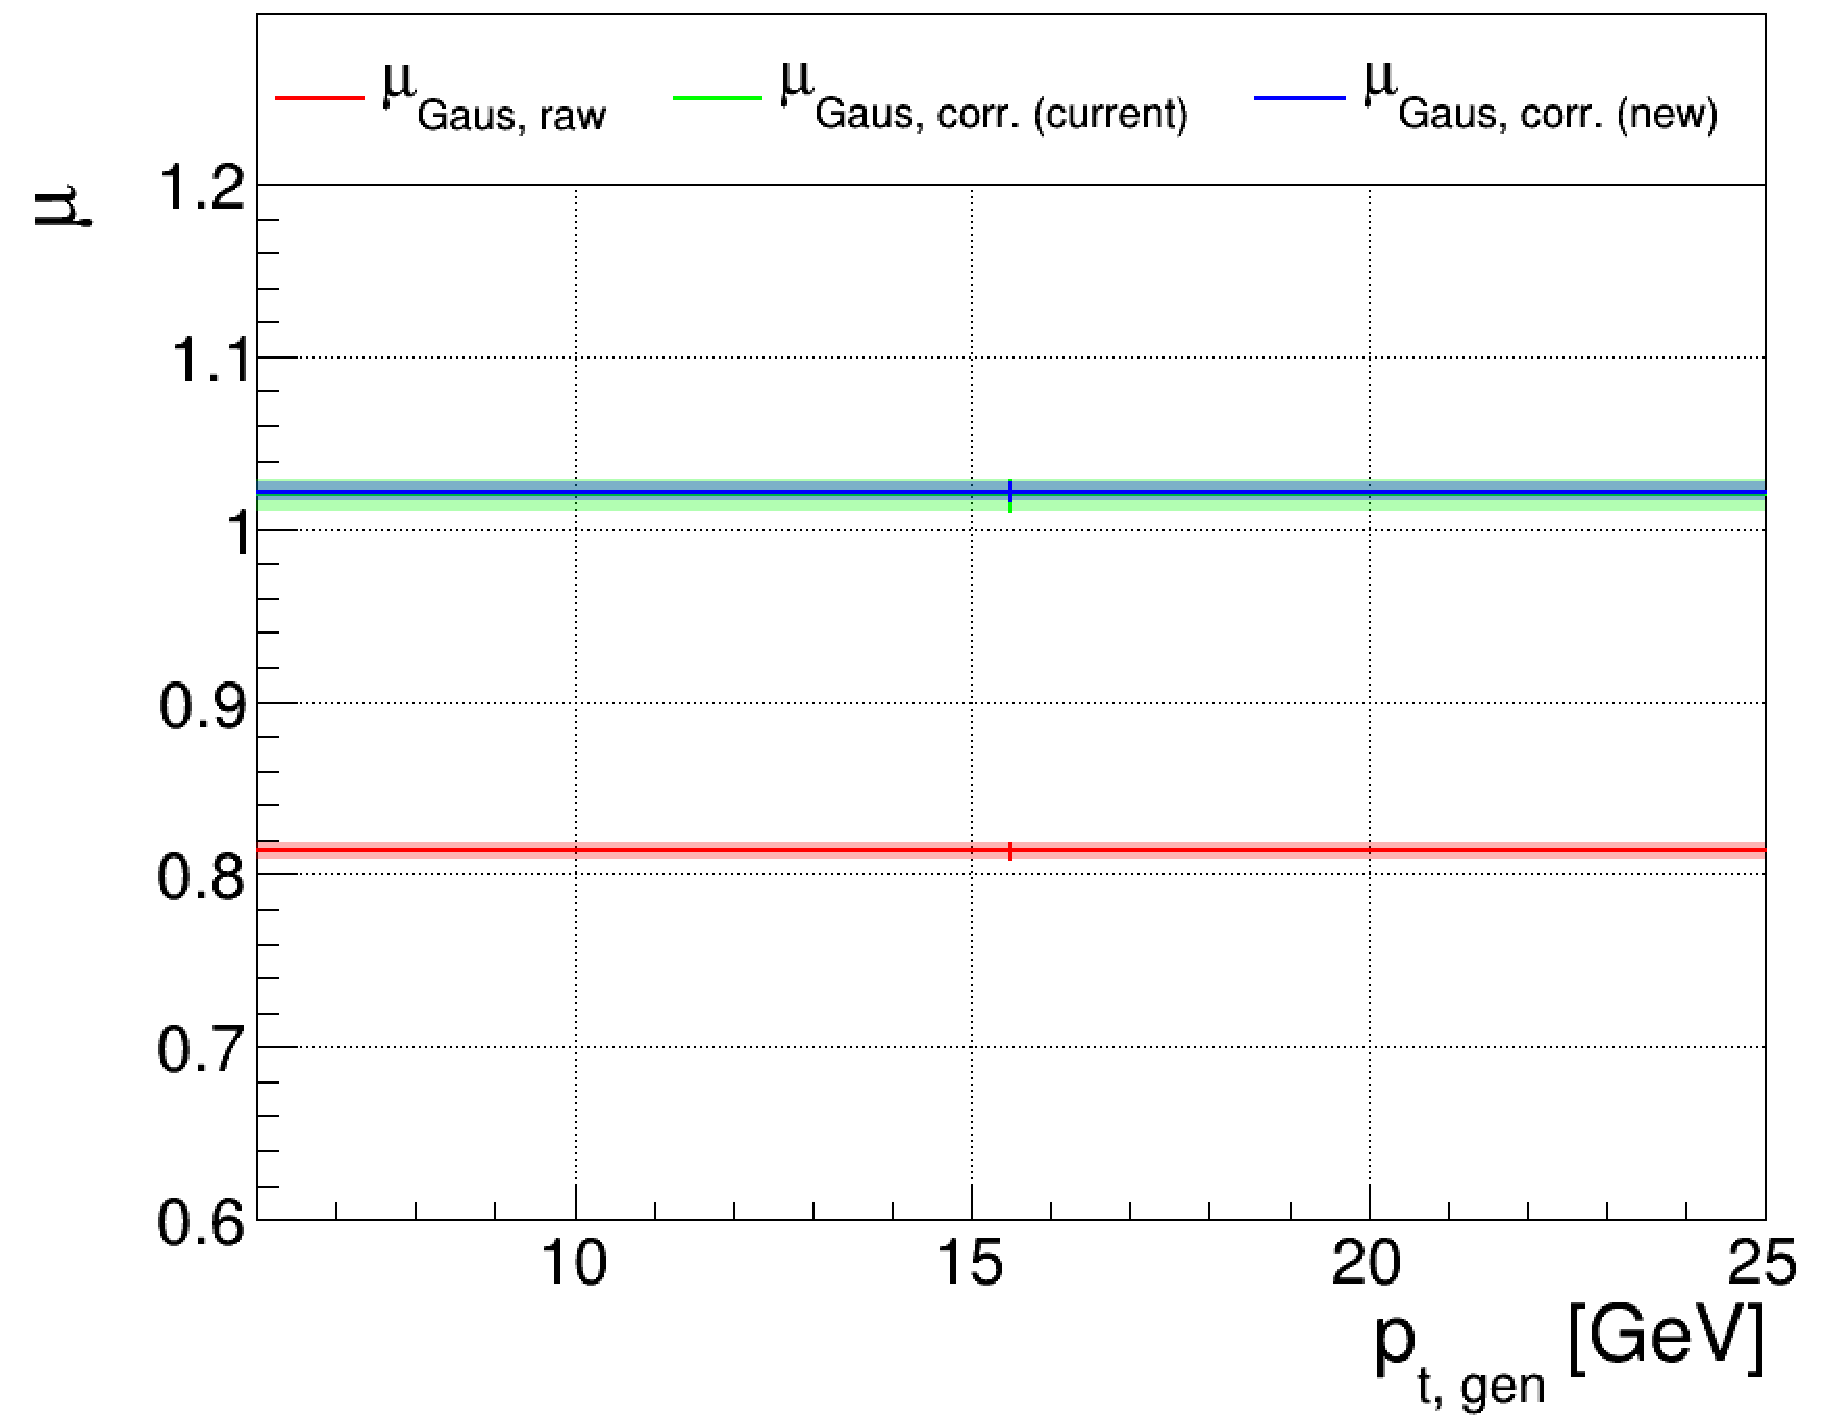
\includegraphics[width=0.495\textwidth]{./plots_pdf/ECAL_plots/plotsPU/EE/ZS/pdf/GENPT/EEZS_GENPT_0006_0025_MuOverBins.pdf}
%% 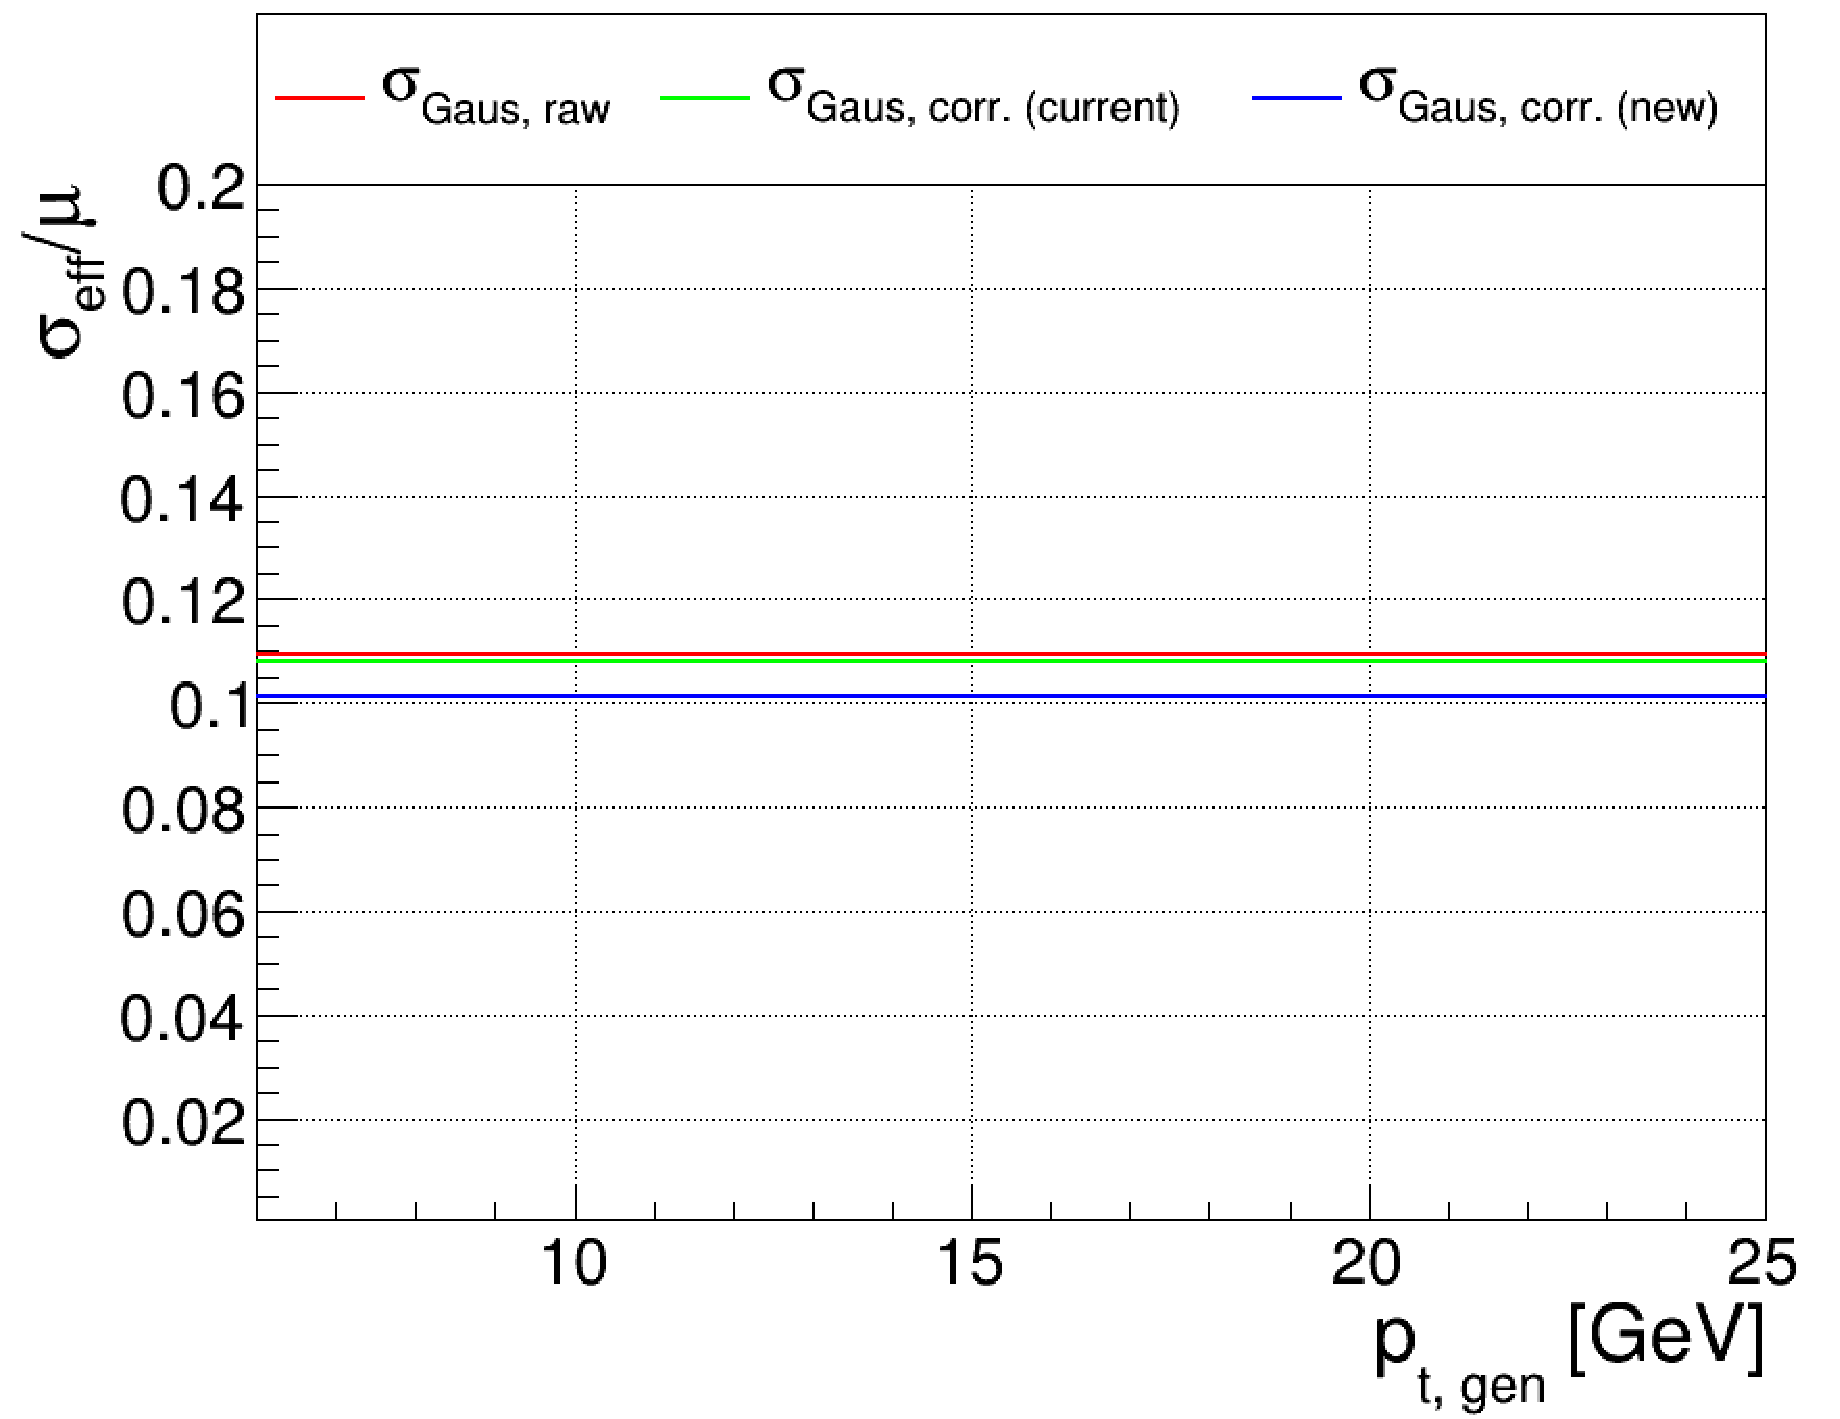
\includegraphics[width=0.495\textwidth]{./plots_pdf/ECAL_plots/plotsPU/EE/ZS/pdf/GENPT/EEZS_GENPT_0006_0025_EffSigmaOverBins.pdf}
%% %\caption{EE - ZS Readout pt 6-25}
%% %\end{figure}
%% %\begin{figure}
%% 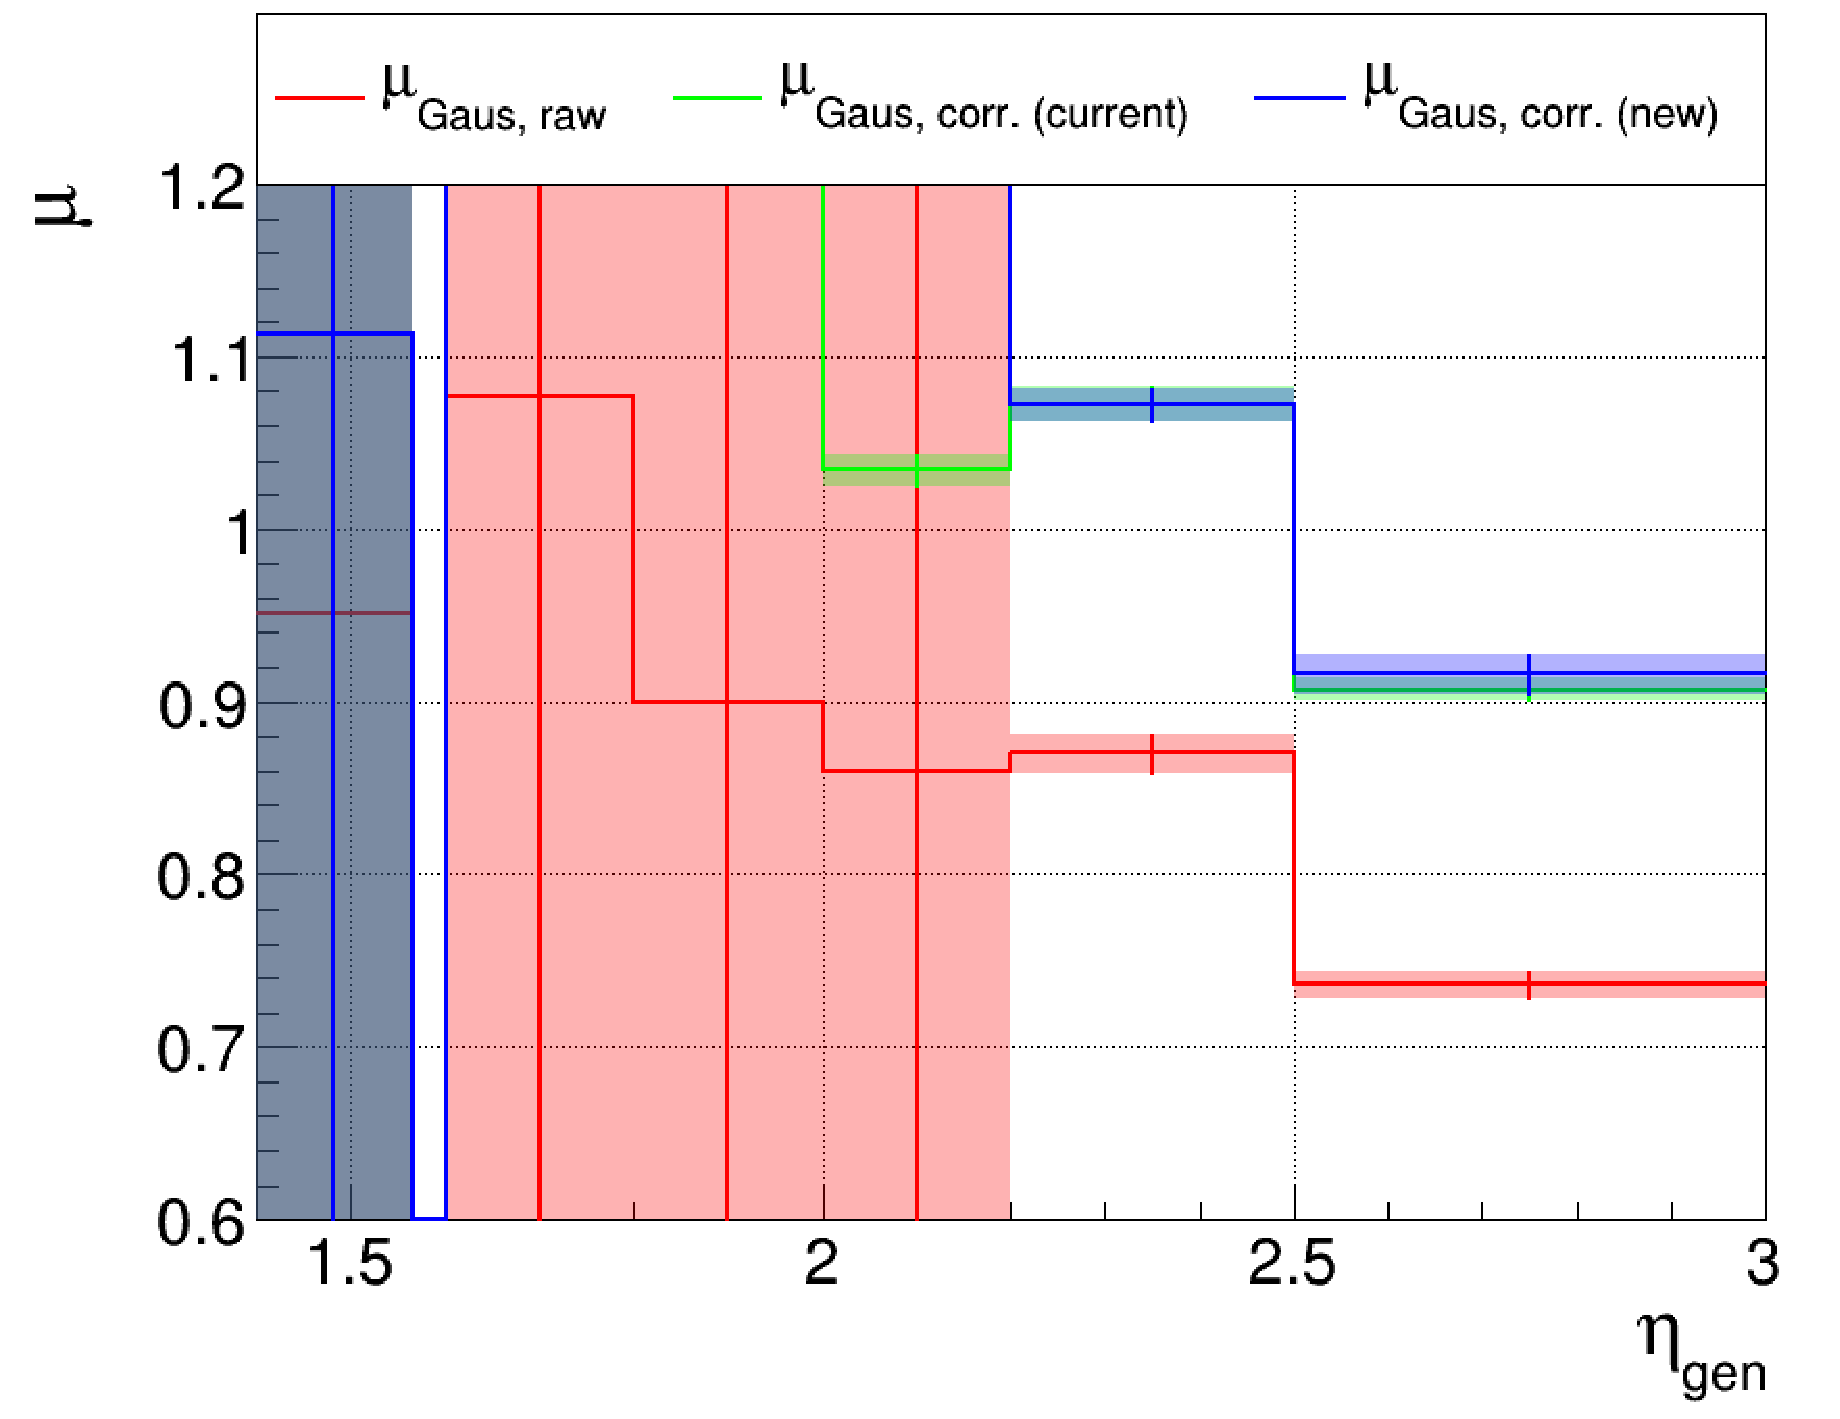
\includegraphics[width=0.495\textwidth]{./plots_pdf/ECAL_plots/plotsPU/EE/ZS/pdf/GENETA/EEZS_GENETA_0006_0025_MuOverBins.pdf}
%% \caption{EE - ZS Readout \pt 6-25}
%% \end{figure}






